\chapter{Chinese Historical Phonology with Marxist Characteristics}
\chaptermark{Marxist characteristics}
\label{chapter-1.-Introduction}

\begin{quote}
während die Methode, vom Abstrakten zum Konkreten aufzusteigen, nur
die Art für das Denken ist, sich das Konkrete anzueignen, es als ein geistig Konkretes zu reproduzieren.
(Marx, Grundrisse)
\end{quote}

%\setlength{\epigraphwidth}{0.8\textwidth}
%\epigraph{...
%we must interrogate the being of the consciousness of science.}{Heidegger, \textit{Being and Time}}
%I CAN'T CONFIRM THIS QUOTE

\section{Baxter and Sagart's new reconstruction}
The 2014 monograph \textit{Old Chinese: A New Reconstruction} by William H. Baxter and Laurent Sagart is the most recent substantially contribution to the reconstruction of Old Chinese. 
Some reviewers, although not entirely uncritical,  greeted this work as a decisive step forward  (\cite{Starostin2015},
  \cite{Goldstein2015},  
  \cite{Hill2017OCreview}), but others 
reject it as unwarranted speculation  (\cite{Schuessler2015BSrv}, 
  \cite{Ho2016}, 
  \cite[]{Harbsmeier2016}).\footnote{Many
  criticisms apply \emph{mutatis mutandis} to all six vowel systems \citep[esp. pp. 183-184]{Ho2016} or even to all efforts in historical
  linguistics \citep[esp. pp. 484-487]{Harbsmeier2016}. The review of \citet[]{Ho2016} inspired several rejoinders \citep{jacques17buyang,Ma2019HoReply, List2016n}. As Max Planck tell us, ``[a] new scientific truth does not triumph by convincing its opponents and making them see the light, but rather because its opponents eventually die and a new generation grows up that is familiar with it'' (\textit{Scientific autobiography}, 1950, p. 33).} 

Before turning to the concrete controversies surrounding the New Reconstruction, let us consider \textit{in abstracto} how a reconstruction can go wrong. Wrong goings may arise either by starting from the wrong evidence base or by a lapse in methodological execution. Since the taking in of all and only the ultimately relevant evidence can in no way be ensured \textit{ex ante}, wrongdoings of the first type we can at last refer to those of the second. Let me illustrate with an example from the work of James Matisoff.\footnote{I offer this example ot from any animus, but simply because of familiarity with the case.} 
Matisoff 
compares Chinese 筆 \textit{pit} 
`writing brush' with Tibetan 
{\tib{པིར་}}
\textit{pir} `writing brush', proposing their descent from a common ancestor \citeyearpar[504]{Matisoff2003}. 
\citet[215]{sagart06review} justifiably points out that this comparison is \textit{prima facie} ridiculous. 

As it is quite impossible that speakers of the Sino-Tibetan Ursprache knew writing brushes, on semantic grounds alone he ought to have left this  comparison outside of his dataset. Matisoff has here done what he ought not to have done. But a scruple about missing out on any valid cognate, might caution one to provisionally include this  comparison, despite its unlikely semantics. I, for one, do not hesitate to compare Tibetan 
√{\sil{l̥ag}} 
({\tib{ཀློག་}} \textit{klog}, past {\tib{བླགས་}} \textit{blags}, fut. {\tib{ཀླག་}} \textit{klag}, imp. {\tib{ལྷོགས་}} \textit{lhog}) `read' with Chinese 讀 \textit{duwk}
< *{\sil{C.lˤok}} `id.', assuming that both underwent the same semantic shift from `intone, chant' to `read' (aloud), after the introduction of the practice of reading into both two societies. 
Nonetheless, 
Tibetan 
{\tib{པིར་}}
\textit{pir} `writing brush' is an obvious loan from Chinese 筆 \textit{pit}. 
Inherited Tibetan words do not begin with unaspirated voiceless stops (\cite{hill07aspirate}) and the correspondence of Chinese -t with Tibetan -r is characteristic of Tang dynasty Chinese loans into Tibetan \citep{Preiswerk2014Alttibetischen}, the correct application of the comparative method could have led Matisoff to remove the comparison from his dataset. By failing to fish out this loanword from his data based on the phonetic correspondences it exhibits, Matisoff has left undone what he ought to have done. This example shows that the sin of omission is graver than the sin of commission; the method, if correctly applied will wash away all errors of data collection.  
In other words, if all performances in the field were methodologically deft, the correct identification of the data explainable through reconstruction would take care of itself.

With the forgoing discussion in mind, it comes as no surprise that it is in their application of method and not in their gathering of data that Baxter and Sagart have irked some readers.\footnote{The critical reviews of \citet{Schuessler2015BSrv}, 
  \citet{Ho2016}, and 
  \citet{Harbsmeier2016} each in their way grudgingly acknowledge that Baxter and Sagart's increased engagement with early Chinese loans into neighboring languages is \textit{per se} a good thing.} 

\section{The Baconians versus the Popperians}
Baxter and Sagart credit their progress, at least in part, to their philosophy of science.  

\begin{quote}
[W]e encounter two diverging views about how linguistic history
is reconstructed. One traditional view is that [...] %[historical linguists have certain scientific
%procedures at hand that, if correctly applied, will produce reliable results and will not lead them into error.
%... 
%Conclusions resulting from the correct application of these methods may be regarded as ``proved.'' (It follows from this view that if two scholars reach different results, one of them--at least--must have applied the methods improperly.)
%Furthermore, in such a view,] 
researchers must go as far as the data take them and no
farther; to speak about matters unseen would be unscientific.
[...]
%It is doubtful whether anyone ever implemented this approach consistently, but this
%is how the process of reconstruction is sometimes described: certain results are said
%to be ``proved,'' and disagreements between researchers are attributed to illegitimate
%procedures on one side or the other. 
An alternate view of scientific inquiry, which we
adopt here, is the hypothetico-deductive approach (as described, for example, in 
\cite[28-29]{Mayr1982}).
%\footnote{Mayr, Ernst. 1982. The growth of biological thought: diversity, evolution, and inheritance. Cambridge, MA: Belknap Press.} 
In our view, a linguistic reconstruction is a set of hypotheses about
the linguistic past. Hypotheses are not simply summaries of observations; crucially,
while they are based on existing observations, they also make testable predictions
about future observations. This is the deductive part of the approach. Hypotheses
cannot be proved, but they can be tested empirically. If the predictions they make are
false, hypotheses can be disproved, and in that case it is the scientist's job to revise
or replace them. \citep[5]{Baxter2014OldChinese}\footnote{Transparency requires that I point out the content of the first ellipsis: ``One traditional view is that historical linguists have certain scientific procedures at hand that, if correctly applied, will produce reliable results and will not lead them into error.'' I hold this traditional view without apology and the goal of this essays is precisely to adumbrate the `scientific procedures’ that in Chinese historical phonology will not lead us to error.}
\end{quote}
Thus, Baxter and Sagart contrast the Baconian approach that they wish to pass beyond with their own embracing of a Popperian methodology. 

The criticisms their book has attracted from avowed empiricists makes clear that Baxter and Sagart are correct to characterize the field as divided into two methodological camps.  





\begin{quote}
%就這個例子來看，
《新論》爲了給自己的一個理論找證據，首先設立一個方法論前提，再去主觀地找材料，只取對自己有利的例子，並且對材料也沒有做正確的分析。這種做法帶有明顯的先入爲主的觀念，用材料來遷就理論，是難以得出正確的結論的。\\
In order to find evidence for one of its theories, the New Theory first establishes a methodological premise, and then subjectively searches for materials, taking only those examples that are favorable to itself, and does not correctly analyze the materials. 
Such an approach is obviously preconceived, and it is difficult to draw correct conclusions when using materials to accommodate theories. (Xiang et al. 2018)
\end{quote}
Put more succinctly ``[f]acts precede and matter more than interpretation'' \citep[183]{Ho2016}. 
The critiques that Kant and Sellars raise against empiricist  are too well known to rehearse here, but we allow a few lines from Lukács by way of reminder.

\begin{quote}
The blinkered empiricist will of course deny that facts can only become facts within the framework of a system -- which will vary with the knowledge desired. He believes that every piece of data [...], every statistic, every raw event already constitutes an important fact. In so doing he forgets that however simple an enumeration of `facts' may be, however lacking in commentary, it already implies an `interpretation'. Already at this stage the facts have been comprehended by a theory, a method; they have been wrenched from their living context and fitted into a theory.
\citep[PAGES]{Lukacs1923}
\end{quote} 


\section{The place of rare observations in science}
Baxeter and Sagart come in for a fair bit of criticism for their concentration on strange phenomena and difficult cases. 

\begin{quote}
從科學研究的角度看，這種只憑極個別例子就歸納出一種理論的做法是非常危險的 \\
From the point of view of scientific research, it is very dangerous to generalize a theory based only on very uncharacteristic examples. (Xiang et al. 2018)\footnote{https://www.sohu.com/a/255340335_488532 (accessed 13 Jan. 2024.)}
\end{quote}
Perhaps it is dangerous (危險) to generalize a theory on the basis of idiosyncratic examples, but within historical linguistics generalizing on the basis of idiosyncratic examples has traditionally been held to be the  practice that leads to truth \citep[27]{Meillet1925}. 
The alternation between -s- in the singular and -r- in the plural seen in the two English verbs \textit{is}/\textit{are} and \textit{was}/\textit{were} was once regular, and to reconstruct the pattern for the proto-language in its entirety on the basis of these two examples would be quite correct. 
The Vedic first person singular athematic middle optative is only attested as -\textit{īya}, but the form *-\textit{iya}, which is three times implied by the meter is the inherited form \citep[]{Gunkel2022iya}.
ADD JAY'S THING ON TOKHARIAN

With the standard practice of historical linguistics in mind, Schuessler's criticism that for Baxter and Sagart a ``piece that does not fit a general pattern is claimed to reflect an original state which is then applied to everything else'' \citep[577]{Schuessler2015BSrv} reads more like a description of best practice. 
Schuessler is disappointed with the importance that Baxter and Sagart put on rare phenomena, because he expects ``
%The marginal as norm. A tendency to argue that the marginal or unlikely represents the norm. 
%A piece that does not fit a general pattern is claimed to reflect an original state which is then applied to everything else, whereas 
%we usually expect 
the common pattern to be taken as the norm \citep[577]{Schuessler2015BSrv}. 
%\end{quote}
Schuessler finds Ice 1h in his freezer and he finds that it cools his lemonade; he sees no need for chemists to bother themselves with the other 18 forms of ice known so far. These aberrant ices are only found at high pressures, low temperatures, and in outer space, hardly the circumstances that should be considered when articulating a scientific norm. The 11 syllable lines of Hamlet's famous soliloquy give Schuessler no pause; Shakespeare usually manages to write 10 syllable lines and it would be quite unscientific to bring to bear his marginal poetic behavior into the judgement of his art overall. 

There are of course circumstances in which the discounting of rare phenomena can be appropriate in scientific practice, but these circumstances are quite constrained. 
Ignoring outlying data points is appropriate when the existence and the distribution of such outliers is itself predicted theoretically. 
In particular, rare phenomena can be safely ignored if their occurrence cannot be reliably distinguished from random chance or from a measurement error. 
Neither Schuessler nor any of the other critics of Baxter and Sagart have attempted to demonstrate that the rare phenomena within their purview are of this type. 

Put simply, accounting for rare events, far from being methodologically inexcusable eccentricity of our two authors, is to a large extent the actual point of science and is certainly a cornerstone of the scientific method. 

\section{The possibility of prediction}
Schuessler, perhaps reluctant to aim a frontal attack on Popper himself, proposes that the hypothetico-deductive approach has a place in the `hard sciences', but that historical linguistics should be left to the Baconians.\footnote{This proposed division of labour is extraordinary in several respects. First, 8 abandons the unity of science as a program--no small sacrifice. Second, it relegates such observational and imminently historical sciences as astronomy and paleontology, which methodologically parallel our own discipline in so many of their particulars, to the “soft sciences”. Third, it disregards that the founders of empiricism were aiming first and foremost at articulating the correct methodology of the hard sciences.}

\begin{quote}
Testing (falsifying) in natural sciences is different from recovering a dead language.
Physics can predict exactly how a body moves, where only one immutable
law needs to be understood. Sounds and meanings can change in unpredictable
ways (*t- > \textit{d}, \textit{th}, \textit{ts}, \textit{s}, \textit{{\sil{ʔ}}}, etc. depending on language, time and place) and can
only be explained \textit{ex post facto}. Explanations are often matters of interpretation,
judgment and plausibility. Then, in the hard sciences hypotheses can be falsified
with repeatable tests; drop an object to falsify gravity. But dead languages have no
native speakers. Predicting the behavior of rhymes in Old Chinese literature is a
matter of interpretation (a rhyme that does not fit may be a bad rhyme, a word may
have been pronounced differently, graphic error, obsolete word). Predicting that a
certain word will not be written in a certain way in manuscripts that may come to
light one day does not seem a viable test or falsification. \citep[577]{Schuessler2015BSrv}
\end{quote}

\begin{quote}
Traditionally the burden
of proof is on the one who makes a claim (B\&S dismiss this kind of ``proof''). The
new method leaves it to the skeptical audience to falsify propositions. \citep[577]{Schuessler2015BSrv}
\end{quote}

\noindent Schuessler too sharply draws the contrast between the hard and soft sciences. 
The major theme in this quotation is the hard sciences can predict the future and the social sciences cannot. Fine, but Baxter and Sagart nowhere proposed to predict what Chinese will sound like in 3,000 years from now, so this element of Schuessler's critique is irrelevant.
\footnote{Schuessler's insistence on Occam's razor loses focus on the caveat \textit{sine necessitate}. If Schuessler thinks, for example that the uvular hypothesis is incorrect, he would do well to propose his own answer to why some \textit{xiéshēng} series mix velar and glottal initials. Simply setting problems permanently to one side is certainly not how science progresses.}

The interpretation of data in the heart sciences is often controversial. Witnessed the slow acceptance of the atomic theory. First proposed by Democritus and only generally excepted after Einstein. The discoveries of labiovelars in Mycenaean Greek, the laryngeal of Hittite, and the cluster -\textit{htk}- in Swamy Cree are examples not unlike that famous 1919 photograph.

In short, Baxter and Sagart are correct distinguish a Baconian empirical and a Popperian hypothetico-deductive approach to science and correct to see the latter as the more advanced of the two period nonetheless, I shall argue below that a third approach to science dash the dialectic approach dash is more advanced still, preserving and combining the advantages of the two lower forms. But, first let us look concretely at how the empiricists and the hypothetico-deductivists wrangle.


\section{Were 工  and 公 homophones in Old Chinese?}

This section, by virtue of its practical focus, must take for granted much of the terminology of old Chinese historical phonology. The reader who prefers to remain at a relatively abstract level until the machinery of Chinese historical phonology has been introduced systematically, may turn to section 
\ref{sec:BnS-philo-sci}.

 On the basis of series that mix readings with Middle Chinese velars (見 \textit{k}-, 群 \textit{g}-, 匣 \textit{h}-, 曉 \textit{x}-) and readings with initial glottal stop (影 '-) or initial 以 \textit{y}-. Baxter and Sagart propose that the fricative (匣 \textit{h}-, 曉 \textit{x}-), glottal (影 '-) and glide (以 \textit{y}-) initials found in such series originate from uvular initials 
 \citeyearpar[43-46]{Baxter2014OldChinese}. 
 They explain velar stops (見 \textit{k}-, 群 \textit{g}-) occurring in the relevant series as arising from complex onsets (pp. 168-170),2 e.g. 公(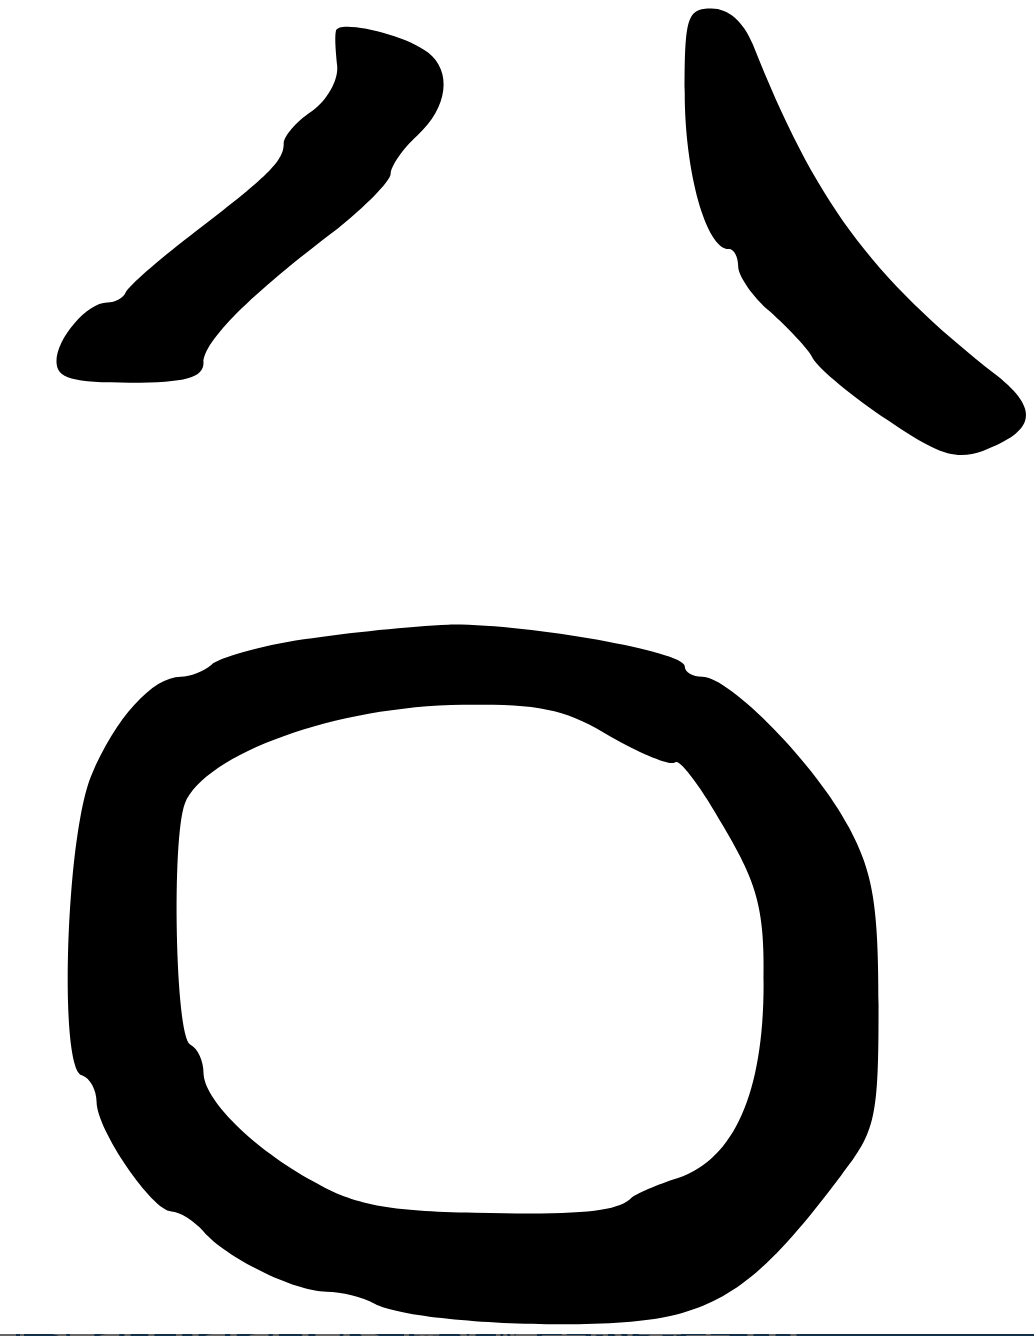
\includegraphics[scale=0.015]{Chapter1/kuwng.png}
 in early texts) \textit{kuwng} < *C.qˤ-, 瓮  \textit{'uwngH} < *{\sil{qˤ-}}, 容(
\includegraphics[scale=0.015]{Chapter1/yowng.png}) yowng < *{\sil{ɢr}}-.\footnote{Unfortunately, their proposals are not sufficiently explicit to allow the reader to predict their reconstruction of a given word. For example, they reconstruct many of the readings in the series built on 貴 with velar initials (e.g. 簣 \textit{khweayH} < *{\sil{kʰˤr}}- and 聵 \textit{ṅweayH} < *{\sil{[ŋ]ˤr}}-), despite the presence of readings such as 潰 \textit{ḫwəyH} and 遺 \textit{ywiy} suggesting a uvular series. Their proposed developments of uvulars occasionally appear phonetically odd. For example, they propose that *m.qʰ-, *m.ɢ-, *N.qʰ-, *N.ɢ- develop to 疑 ng-, whereas *m.q- and *N.q- merge with *ɢ-. Nonetheless, the clear-cut correspondence of Chinese uvulars to Tibetan velars and Burmese zero onset (e.g. Chi. 箴 \textit{cim} < *{\sil{t.qəm}} `needle', Tib. 
{\tib{ཁབ་ }}
\textit{khab}, 
Bur. 
{\burm{အပ်}} \textit{ap}; Chi. 窨  \textit{'imH} < *{\sil{q(r)[ə]m-s}} `subterranean room`, 
Tib. 
{\tib{ཁྱིམ་}}
\textit{khyim} `home', Bur. 
{\burm{အိမ်}} 
\textit{im}; Chi. 縊  \textit{'eyH} < *{\sil{qˤik-s}} `strangle', Tib.
{\tib{འཁྱིག་}}
\textit{ḫkhyig} `tie, fasten, suffocate', Bur. 
{\burm{အစ်}}
ac 'squeeze, throttle', etc.) versus velars in all three languages (Chi. 苦 \textit{khuX} < *{\sil{kʰˤaʔ}} `bitter', Tib. 
{\tib{ཁ་}}
\textit{kha}, Bur.
{\burm{ခါး}} \textit{khāḥ}; Chi. 岡 \textit{kang} < {\sil{*kˤaŋ}} `hill', Tib. 
{\tib{སྒང་}}
\textit{sgaṅ}, Bur. 
{\burm{ခင်}} \textit{khaṅ}, etc.) convincingly confirms the correctness of the Old Chinese uvular hypothesis.}  

Several reviewers take umbrage with this proposal. Let us start with Peking.\footnote{https://www.sohu.com/a/255340335_488532}

\begin{quote}
%《新論》認爲``工''和``公''在中古是同音字，以往的學者認爲在上古它們也是同音，但是在先秦文獻中，``工''和``公''沒有出現混用的例子，這說明它們在先秦不同音，因此``工''構擬成*kˤoŋ，``公''構擬成*C.qˤoŋ，這樣也能解釋以``公''爲主諧字的諧聲字都有小舌音聲母[1]。
%
%按：《新論》中的這個論斷是基於作者的一個方法論前提，即語音構擬不僅要解釋已經出現的現象，也要解釋爲什麼有些現象不能出現。例如在談到上古漢語韻文材料的時候，他們說：``一個合理的上古音構擬的要求之一就是要能解釋在《詩經》里哪些字能互相押韻，並且同樣重要的是要能解釋哪些字不能互相押韻。''[2]從擬音是否客觀反映韻部遠近的角度看，這個看法大體是正確的，而且我國學者很早就在他們的研究中體現了這個觀點。例如段玉裁分古韻爲十七部，他雖然沒法用國際音標爲每個韻部構擬音值，但是卻按照心目中音值的遠近來排列韻部，他把古韻十七部分爲六大類：之部是第一類；宵幽侯魚音近，是第二類；蒸侵談音近，是第三類；東陽耕音近，是第四類；真文元音近，是第五類；脂支歌音近，是第六類。拿我們今天的古音構擬成果來看，段玉裁的這種安排也是比較合理的，它能夠解釋古書中的合韻、音轉等現象，也就是哪些韻部相近，但同時也能解釋韻部相遠的現象，例如先秦魚部和宵部相差甚遠，往往不能一起押韻，段玉裁雖然將它們同列第二類，但分居首尾，說明段玉裁認爲它們讀音仍然有較大區別[3]。段玉裁對先秦韻部的這種安排是根據對材料的精細考察、分析而得出的，所以具有科學性。
%
%然而反觀《新論》，其中很多推理都值得進一步推敲，不能接受材料的檢驗。例如書中認爲``五''和``午''是兩個常見的聲符，但是在先秦它們沒有出現相通的情況，直到《說文》時代才有交替的例子，這說明它們先秦不是同音字，因此《新論》把``五''的聲母構擬爲*C.ŋˤ-，把``午''的聲母構擬爲*m.qhˤ-[4]。最近何大安先生在給《新論》所作的書評中詳細地批駁了這個看法，指出至晚在西周晚期就有``五''和``午''相通的例子。何先生認爲《新論》這個推理的問題主要有兩點：一是我們依據的往往是不全面的材料（incomprehensive materials），因此有些語言現象沒有反映出來，但沒反映（not attested）並不一定代表不存在（not existed）；二是《新論》往往只依靠一些工具書，而沒有親自去查閱原始材料。針對這種情況，何先生還特別引用了趙元任先生給王力先生《中國古文法》的評語``言有易，言無難''[5]，發人深省。

此處《新論》對``工''、``公''的處理同樣存在問題。我們也查閱了一些《通假字典》類的工具書，發現在《新論》設定的上古音範圍內（即公元前221年秦統一中國之前），目前確實沒有找到``公''、``工''混寫的情況。這可能有兩種情況，一是確實先秦``公''和``工''不相通；二是目前保存的先秦文獻較少，``公''、``工''先秦就有相通的情況，只不過文獻沒有記錄下來（not attested），至少沒有被收入到這些工具書當中。這都有待對材料進一步發掘才能得出確鑿的結論。 \\

Here, the treatment of 工 and 公 in the New Theory is also problematic. We have also checked some reference works such as the 通假字典 \textit{Tōngjiǎ zìdiǎn} (ADD CITATION) and found that there is no mixed use of 工 and 公 in the range of ancient sounds set by the "New Theory" (i.e., before the Qin unified China in 221 B.C.). This may be due to two reasons: firstly, it is true that 工 and 公 were not mutually compatible in the pre-Qin period; secondly, there are relatively few pre-Qin documents preserved, and 工 and 公 were mutually compatible in the pre-Qin period;  
it is only that they are not attested in the relevant literature, or at least, not in these reference works. All this requires further exploration of the material to draw a definite conclusion.
\end{quote}

Suppose for a moment that the proposal of Baxter and Sagart is correct; no amount of further exploration of the material will allow us to draw a definite conclusion. Newly discovered pre-Qin documents and newly compiled reference works will continue to fail to find any phonetic contact between 工 and 公.   
It is incumbent on the skeptic to stipulate what evidence he requires to change his mind. Otherwise, it is he, and not Baxter and Sagart, who is dogmatically married to \textit{a priori} assumptions; the proposal that 工 and 公 were always homophones is itself unfalsifiable. 

By drawing attention to the small size of the pre-Qin corpus in comparision to the Han corpus, 
the Pekin skeptic implies that he would find the new propsoal convincing if the corpus of pre-Qin documents happened to exceed the Han corpus in size.\footnote{Although he could still insist that the absence of evidence for contact between 工 and 公 was due entirely to change.} 

We could use statistics to at least parameterize this difference of opinions. How many characters occur in the entire Han corpus? How many characters is the entire pre-Qin corpus? How frequent are phonetic loans in each corpus? What are the typical overall frequencies of two chracters that are well attested as phonetic loans for one another in both corpora?  
The Peking skeptic does not raise let alone answer these questions.

DOES THE 通假字典 INCLUDE BOTH PRE-QIN AND HAN MATERIAL?

If Baxter and Sagart had shown that, 工 and 公 are both frequent enough that, based on parallel cases, one expects a certain amount of phonetic loaning among them, this would be good, but the Peking school would probably continue to find grounds for grumbling. Both sides should put their cards on the table and stipulate how in principle they think it is possible to separate signal and noise. 

In his 1992 book Baxter put his cards on the table very explicitly. 
In his \textit{Handbook} he went to great length to argue that certain failures of characters to rhyme disproved earlier understandings of the Old Chinese vowel system. 

I NEED TO SUMMARIZE HIS APPROACH 

\begin{quote}
    Schuessler believes that Baxter (1992) did not use hypothetico-deductive thinking. On the contrary, in classic hypothetico-deductive manner, that work formulated two hypotheses about OC rhyming: the rounded-vowel hypothesis and the front-vowel hypothesis, which predicted that certain types of rhyming, hitherto judged lawful, did not in fact exist in statistically significant numbers. Statistical testing by Baxter confirmed the two predictions, supporting both hypotheses. \citep[]{Baxter2017schuess}
\end{quote}

They base it on the basis of X series that one is k- and one is q-. This predicts that they should not have tongjia relationships (until uvulars and velars merge closed parentheses. This prediction is borne out by the philological evidence. The opponent says it is simply due to a positive evidence. This poses the methodological question of how much data one needs in order to show that something has not happened. This is actually where popper is helpful. The hypothesis has been tested and has passed the test. This means nothing except that the hypothesis should be allowed to live for another day.



\begin{quote}
%但至晚在漢代，``公''、``工''相通的例子就已經比較普遍了，這也同漢代流傳下來的文獻更多有關係。《史記·封禪書》：``受此書申公。''《孝武本紀》``申公''作``申功''，``功''从``工''得聲。《詩·大雅·靈台》：``蒙瞍奏公。''《楚辭·九章》``矇瞍謂之不章''王逸注引《詩》作``蒙瞍奏工''，《呂氏春秋·侍君覽·達鬱》``矇箴師誦''高誘注引《詩》作``矇叟奏功''。
也許有人會爲《新論》辯護，認爲先秦沒有出現``公''、``工''相通的例子，而漢代有這種情況，這可能是因爲到了漢代兩字讀音才變得相同。我們認爲這個看法不能成立。首先，目前我們沒有找到先秦``公''和``工''聲母讀音不同的內證材料，研究上古音，必須充分利用一切反映上古語音面貌的內證材料，尋求科學合理的解釋，就筆者目力所及，目前所有直接的內證材料都沒有顯示出``公''、``工''讀音有別，那麼有些人認爲它們先秦不同音便沒有充足的理由。
%第二，王力先生《漢語語音史》在談到漢代音系時說：``關於漢代的聲母，我們沒有足夠的材料可供考證，這裏缺而不論。可以假定，漢代聲母和先秦聲母一樣，或者說變化不大。''[6]這是在仔細研究材料后得出的實事求是的結論，如果沒有堅強的理由，我們不能輕易拋棄。上面我們引了漢代``公''和``工''相通的例子，說明那時它們讀音就相同或相近，書面語要滯後於口語，那麼很可能先秦口語中它們讀音就是一樣的。第三，文字相通的成因是複雜的，《新論》把這個問題想得太簡單，也暴露出作者在基礎知識和邏輯推理上的漏洞。如果兩個字有通假的情況，並不能就此認爲它們的讀音一定相同，有可能是由於字形相似造成的誤寫，因爲詞義的引申而新造一個分化字，分化字和本字也可能會出現相通的現象；相反，即使兩個字讀音相同，它們也不一定會相通。其實我們只要看看郭錫良先生的《漢字古音手冊》（增訂本）就會發現，中古和上古都同音但在上古卻不相通的字有很多，例如``畢篳蓽韠䟆蹕滭㪤㓖熚彃㮿縪罼必珌''中古都是幫母質韻字，上古同屬幫母質部，但是先秦文獻中``畢篳蓽韠䟆蹕滭㪤㓖熚彃㮿縪罼''等字不與``必珌''相通，
%它們分屬兩個諧聲系列；又如``暄萱諼吅喧諠䚭䚙''中古都是曉母元韻字，上古同屬曉母元部，但先秦文獻中``吅''和其他字不相通，它們分屬不同的諧聲系列。這樣的例子還有很多，《新論》爲什麼不按照處理``公''、``工''那樣的辦法來爲它們構擬不同的上古音呢（在《新論》里，``吅諠喧''的上古音都是*qwhar）？這難道不是自相矛盾嗎？究其原因，還是在於他們這樣做的目的。《新論》之所以非要認爲``公''和``工''上古讀音不同，是要以此作爲所謂``小舌音假設''（uvular hypothesis）的證據，在《新論》的上古音系統里，共有四套小舌音聲母，這個構擬在白一平和沙加爾之前的文章中有論述，他們認爲當一個特定的韻類中有兩個對立的諧聲系列、並且它們在中古有同樣的舌根音聲母時，通常情況是其中一個系列在上古是小舌音，也就是``舌根音+ʔ-、x-、h-''的形式，另一類則是普通的舌根音，他們舉出了主元音是-o-的四個例子：``冓：句''、``侯：后''、``工：公''、``角：殻''，每個配對中的前一個是舌根音聲母，後一個是小舌音聲母[7]。關於這個假設，我們可以再討論，但至少``工：公''這個例子是不能成立的，那也就是說所謂的小舌音假設是存在漏洞的。

Perhaps some people will defend the "New Theory", arguing that there is no example of 公 and 工 in the pre-Qin Dynasty, but there was such a situation in the Han Dynasty, probably because the pronunciation of the two characters became the same in the Han Dynasty. We think this view is not valid. First of all, we have not found any internal evidence for the different pronunciation of the vowels of 公 and 工 in the pre-Qin Dynasty. As far as I can see, all direct internal evidence does not show that 公 and 工 are pronounced differently, so there is no good reason for some people to think that they sound different in the pre-Qin period. 
%Secondly, Mr. Wang Li's "History of Chinese Phonology" says about the phonology of the Han dynasty: "We do not have enough material to verify the phonemes of the Han dynasty, which are not available here. It can be assumed that the vowels of the Han dynasty were the same as those of the pre-Qin dynasty, or that they did not change much." [6] This is a pragmatic conclusion reached after careful study of the materials, and we cannot easily discard it without strong reasons. We have cited above the example of the Han Dynasty when the words "Gong" and "Gong" were pronounced the same or similarly, and the written language lagged behind the spoken language, so it is likely that they were pronounced the same in the pre-Qin oral language. Thirdly, the causes of textual congruence are complex, and the "New Theory" makes this issue too simple, revealing the author's gap in basic knowledge and logical reasoning. If two words have the same pronunciation, it cannot be assumed that they must have the same pronunciation. It is possible that the misspelling is caused by the similarity of the characters, and that a new differentiated word is created because of the derivation of the meaning of the word, and the differentiated word and the original word may also have a common phenomenon. In fact, if we look at Mr. Guo Xiliang's Handbook of the Ancient Pronunciation of Chinese Characters (updated version), we will find that there are many characters that have the same pronunciation in both the Middle Ages and the Upper Ages but do not share the same pronunciation in the Upper Ages. The Middle and Early Dynasties are both "譯必珌", and the Upper Dynasties are in the same part of "蔣".  However, in the pre-Qin dynasty literature, the word "ㄅ" and other characters are not related to each other, and they belong to different harmonic series. There are many other examples of this kind, so why didn't the XINLU follow the same way of "Gong" and "Gong" to construct different ancient sounds for them (in the XINLU, the ancient sounds of (in the New Discussions, the ancient sound for "meaning" is *qwhar)? Is this not a contradiction? The reason for this is because of the purpose of doing so. The reason why the New Theory has to argue that the ancient pronunciation of "Gong" and "Gong" are different is to use this as evidence for the so-called "uvular hypothesis". They argue that when there are two opposing harmonic series in a given rhyme class and they have the same lingual root vowel in the Middle Ages, it is usually the case that one of the series is lingual in the Upper Ages, i.e., "lingual root vowel + ʔ-, x-, h-", and the other is the common lingual root consonant, and they give four examples where the primary vowel is -o-: "冓: 句", "侯: 後", "工: 工 The first one in each pair is a lingual root vowel and the last one is a small lingual vowel [7]. We can discuss this assumption again, but at least the example of "Gong: Gong" is not valid, which means that there is a loophole in the so-called ligular vowel assumption.
\end{quote}

Well, the are of course not mentioning the reason given by Baxter and Sagart, namely to explain contact between velars and glottals in certain xiéshēng series. 

Here I want to quote Zurcher, p. 269, who has a great discussion of the \textit{argumentum ex silencio}

SEE WHAT SCHUESSLER SAYS ABOUT 公 and 工



\begin{table}[]
    \centering
\makebox[\textwidth]{\begin{tabular}{lllllll}
\hline
    & MC & Karlgren & Pan & S\&B & OCM & Outside connections \\ \hline
    公 gōng ``uncle'' & {\sil{kuŋ}} & *kung & *{\sil{klooŋ}} & *{\sil{C.qˤoŋ}} & *{\sil{klôŋ}} & Tai {\sil{luŋ}}A² ``uncle'' \\ 
翁 wēng ``old man'' & {\sil{ʔuŋ}} & – & & *{\sil{qˤoŋ}} & (*{\sil{ʔôŋ}}) & Lushai unL ``elderly'' \\ 
瓮甕 wèng ``jar'' &  {\sil{ʔuŋ′}} & *{\sil{ʔung}} & *{\sil{qlooŋs}} & *{\sil{qˤoŋ-s}} & *{\sil{ʔôŋh}} \\
\makecell[l]{
訟 sòng ``litigate'' \\
= 誦 ``admonish''} &
{\sil{zjwoŋ′}} & *{\sil{dziu̯ ng}} & *{\sil{sɢloŋs}} & *{\sil{s-ɢoŋ-s}}  & *{\sil{s-loŋh}} & WT {\sil{luŋ}}
``admonition'' \\
松 sōng ``pine tree'' & {\sil{zjwoŋ}} & *{\sil{dziu̯ng}} &  
*{\sil{sɢloŋ}} & *{\sil{sə.ɢoŋ}} & *{\sil{s-loŋ}} \\
崧 sōng ``high'' & {\sil{sjuŋ}} & *{\sil{siô̯ng}}
& 嵩 *{\sil{suŋ}} & *{\sil{[s]uŋ}} & *{\sil{sluŋ}} & PMK *{\sil{sluuŋ}} ``high'' \\
妐 zhōng
``father-in-law'' &
tśjwoŋ &&& *t-qoŋ & *toŋ \\
\hline
    \end{tabular}}
    \caption{Phonetic series gōng 公 (apud \citet[]{Schuessler2015BSrv}}
    \label{tab:my_label}
\end{table}


\begin{quote}
The preference to err on the side of complexity results in the NOC reconstruction
of prefixes and initial consonant clusters for several reasons: (a) to make another
hypothesis work, e.g., in order to maintain the uvular hypothesis, a MC k in their
uvular series is derived from a cluster *C.q- (e.g., \textit{gōng} 公 MC \textit{kuŋ} < *{\sil{C.qˤoŋ}} ~ \textit{wēng}
翁 MC \textit{\sil{ʔuŋ}} < *{\sil{qˤoŋ}}); (b) consonant clusters with prefixes as a result of the authors`
view on the phonetic information extractable from graphs; (c) Old Chinese loans
in southern languages; (d) Min dialect data; (e) morphological hypotheses. {\citep[782]{Schuessler2015BSrv}}
\end{quote}

\begin{quote}
B\&S discuss the phonetic series gōng 公 which has the same types of MC initials,
plus MC ʔ (B\&S p. 28f. and elsewhere). Their uvular theory solves the ``intractable
problem'' why the two homophonous gōng series 公 and 工 show no overlap
in writing, i.e., gōng 工 was a plain *K-initial series, while gōng 公 was a Q-series
(Table 5). Thus their uvular theory + prefix theory solved this problem.

Alternative: 工 was reserved for simple K- words, whereas the gōng 公 series had
complex initials with clusters, such as gōng 公 ``uncle'' actually OC *klôŋ, to be connected
to Tai luŋA² ``uncle'' (for the medial *l, cf. sōng 松 *s-loŋ ``pine tree'' which
is phonetic in sōng 崧 *sluŋ ``high'', cf. Proto-Mon-Khmer *sluuŋ ``high''), while
Lushai un and Written Burmese hông could be more plausibly cognates of wēng
翁 *ʔôŋ ``old man''. (The existence and potential relevance of Tai lung and wēng 翁
 Axel Schuessler
are not discussed.) The authors conclude that with their proposal ``there is no need
for *l-clusters in these words'' (S\&B 2009: 233); but one could just as well turn the
argument on its head and say that the alternative suggestion eliminates the need
for uvulars (*l-clusters have typological parallels in Tibeto-Burman and other language
families in the area, but uvulars do not). This alternative could explain just
as well why the two gōng have been kept apart. Another case discussed by B\&S to
demonstrate that point is wǔ 五, 午 and chǔ 杵, cited as Example (2) above.
\end{quote}

Ma deals with wǔ 五 and 午. 
In 2017, Baxter and Sagart say rather more about uvulars, including a discussion of  公, a lot of it from word families. 




\section{Immodesty}
Several reviewers object to what they see as an immodesty in Baxter and Sagart's work. 

\begin{quote}
Maybe in the end we should be modest, and
content with what is actually knowable and plausible about that distant language.    \citep[596]{Schuessler2015BSrv}
\end{quote}

\noindent Modesty is perhaps a laudable civil virtue, but in Science it has no place. 
I rejoice that Galileo, Noether, and Darwin did not hide their lights under a bushel, but set other virtues above modesty.

According to Ho, Baxter and Sagart 
``deviate from received truths'' 
(2016: 117), which, despite Ho's intention, is indeed praise high for a work in science. As Lowell tells us: 

\begin{verse}
New occasions teach new duties; \\
Time makes ancient good uncouth; \\
They must upward still, and onward, \\
Who would keep abreast of truth.
\end{verse}

The point about the folloiwng quote is that it is quite explicit about Schuessler promoting a bottom-up, empiricist approach, in contrast to Baxter and Sagart who take a top down, deductive approach. 
    
\begin{quote}
Uvularists approach the issue from the writing angle, the phonetic series, and then adjust Old Chinese with the aid of theories, rather than starting with what is known about the language and using regular patterns of the writing system for adjustments, putting the cart before the horse.     \citep[PAGE]{Schuessler2015BSrv}

\end{quote}


\section{Baxter and Sagart's philosophy of science}
\label{sec:BnS-philo-sci}
LOOK AT WHERE THE REVIEWERS DISCUSS POPPER


Rejecting the one-sided empiricism of earlier investigators, they instead commit to the `hypothetico-deductive approach'. 

\begin{quote}
[W]e encounter two diverging views about how linguistic history
is reconstructed. One traditional view is that historical linguists have certain scientific
procedures at hand that, if correctly applied, will produce reliable results and will not
lead them into error.
... 
%Conclusions resulting from the correct application of these methods may be regarded as ``proved.'' (It follows from this view that if two scholars reach different results, one of them--at least--must have applied the methods improperly.)
Furthermore, in such a view, researchers must go as far as the data take them and no
farther; to speak about matters unseen would be unscientific.
...
%It is doubtful whether anyone ever implemented this approach consistently, but this
%is how the process of reconstruction is sometimes described: certain results are said
%to be ``proved,'' and disagreements between researchers are attributed to illegitimate
%procedures on one side or the other. 
An alternate view of scientific inquiry, which we
adopt here, is the hypothetico-deductive approach (as described, for example, in Mayr
1982:28–29). In our view, a linguistic reconstruction is a set of hypotheses about
the linguistic past. Hypotheses are not simply summaries of observations; crucially,
while they are based on existing observations, they also make testable predictions
about future observations. This is the deductive part of the approach. Hypotheses
cannot be proved, but they can be tested empirically. If the predictions they make are
false, hypotheses can be disproved, and in that case it is the scientist's job to revise
or replace them. \citep[5]{Baxter2014OldChinese}
\end{quote}



Baxter and Sagart may be ideologically committed to the hypothetico-deductive approach, but they do not in fact pursue it; nor should they. 


\begin{quote}
這顯然是強材料以就我，先假定一個演變機制，再去挑選一些看似合適的材料來論證。\\
This is obviously a strong material for me, assuming an evolutionary mechanism first, and then selecting some seemingly appropriate material to argue.
\end{quote}

I think this guy has a point. They do not look for things to falsify their theory, instead they collect anecdotal support for their theory and leave it to us to falsify it. I do not think there is anything wrong with their method, but it is not Popperian. 

%
\begin{quote}
%歸根結底，在於《新論》作者沒有踏踏實實地深入到漢語文獻內部，沒有仔細地爬梳材料，因此得出的一些看似很巧妙新穎的結論往往得不到材料的支持，
%有些更是無異於空中樓閣。
有些更是無異於空中樓閣。
%\\

%In the final analysis, the author of the New Theory did not go deep into the Chinese literature and did not carefully comb through the materials, so that some seemingly clever and novel conclusions were often not supported by the materials, and 
some of them are 
no more than castles in the air. 
\end{quote}

\begin{quote}
%... Linguistic reconstructions, then, are not simply summaries of observed data;
%rather, they are sets of hypotheses about actual languages--hypotheses that are
%broadly consistent with observed data but that also make predictions about data
%not yet seen. 
Our Old Chinese reconstructions make predictions about what kinds
of rhymes should and should not occur in texts that are either newly discovered
or not thoroughly analyzed; about how words should or should not be written in
documents from the Old Chinese period; and about what pronunciations should or
should not be found in Chinese dialects or in early Chinese loanwords into other
languages. Thus our reconstructions are subject to falsification by either existing or
newly discovered evidence.
\citep[5-6]{Baxter2014OldChinese}
\end{quote}


DISCUSS HOW NOHARA HAS CONFIRMED SOME OF THEIR RECONSTRUCTIONS, AND HOW GUILLAUME AND XUN HAVE EITHER CONFIRMED OR SUPERCEDED THEM. OF COURSE THIS ONLY SHOWS THAT THE RECONSTRUCTION OF INDIDIVUDAL MORPHEMES IS FALSIFIABLE, BUT THAT IS FINE, THE EMPIRICISTS MIGHT NOT LIKE IT, BUT AS A RESEARCH PROGRAMME IT ISN'T NECESSARY THAT THEIR WORK IS FALSIFIABLE. 

MY EXAMPLES REGARDING VAR SUGGEST THAT FALSIFIABILITY IS NOT THE POINT 

If their  hypotheses yield testable predictions, one expects them to state these predictions and specify exactly how to test these hypotheses. Their book contains no statements of the type `if, such and such a word in such a such a dialect is found to be pronounced in such a such a way, this will prove that Old Chinese had an pre-initial *p-.'  
Thus, the famous photograph of a solar eclipse taken on May 29, 1919, 
which Baxter and Sagart invoke as an instance of the hypothetico-deductive approach in action, is an inapt comparison to their actual practice. 

The scientist does not propose and then test hypotheses. Instead, in the course of his practice he discovers abstractions; one could equivalently say that he creates them. He then traces these abstractions in thought as they unfold into their concrete realizations. A theory is proven when other scientists are themselves able to reproduce in their own experience this ascent from the abstract to the concrete. Thus, reproduction is as much a question of psychic guidance as of instrumental replicability. Whether it be a mathematical proof or a series of experiments in a chemical laboratory the logic is the same.

In the following passage we see the subject-object dualism still baked into the hypothetico-deductive approach. 

\begin{quote}
The question how it happens that a new idea occurs to a man---whether it is a musical theme, a dramatic conflict, or a scientific theory---may be of great interest to empirical psychology, but it is irrelevant to the logical analysis of scientific knowledge. \citep[31]{Popper1959logic}
\end{quote}

\begin{quote}
To what extent scientists actually employ the hypothetico-deductive approach is arguable. Collingwood (1939) has stated quite correctly that a hypothesis is always a tentative answer to a question and that the posing of a question is really the first step on the path toward a theory. The history of science knows scores of instances where an investigator was in the possession of ail the important facts for a new theory but simply failed to ask the right question. Accepting the importance of questions, however, im­ mediately leads to new doubts: Why, in the first place, was the question raised? The answer must be because a scientist observed something which he did not understand or something the origin of which puzzled him, or because he encountered some seemingly contradictory phenomena from which he wanted to remove the contradiction. In other words, observations of facts gave rise to the questions. (Mayr 1982 : 29)
\end{quote}

\section{Three approaches to science}

Popper, Kuhn  

In the terminology of György Lukács, Baxter and Sagart rightly criticize the blinkered empiricist, but only from the standpoint of the sophisticated opportunist; they have not yet arrived at orthodox Marxism.


Robert Brandom's terminology of
\textit{bimodal hylomorphic conceptual realism} helps elucidate the methodological requirements of orthodox Marxism. 

\begin{quote}
This is the view that conceptual content shows up in two different
forms, which
are distinguished by the modality of the relations of incompatibility and consequence.
Determinate objective states of affairs are conceptually contentful
in standing to one another in alethic modal relations of noncompossibility
and necessitation. Determinate subjective thoughts express the same conceptual
contents by standing to one another in deontic modal relations of normative
preclusion and consequential commitment.
\citep[109]{Brandom2019Spirit}
%Brandom 2019, p. 109
\end{quote}

SEE IF HE STATES IT MORE ELEGENTLY ELSEWHERE

Only in light of bimodal hylomorphic
conceptual realism is ``the conceptual reproduction of reality'' (Lukács) made possible.

Brandom offers the philosophical starting point, the prerequisite for valid knowledge. To actually make progress in science, we need to add Lukács' emphasis on a totality in historical movement. 

In fact, as described by Kuhn, although not under this name, this is the only method that leads to achievements in science. 

If we return to the uvular hypothesis, we see that 
 Pan proposes uvulars largely on the basis of Sino-Tibetan parallels and early transcriptions of foreign words, but points out resulting improvements in the behaviour of phonetic series. 
 Baxter and Sagart get their ideas from the world; they are not born like Athena directly from their heads. 


\subsection{Empiricism}

\subsection{The hypothetico-deductive method}

\subsubsection{A few quotes from Feyerabend}

\begin{quote}
    The idea of a method that contains firm, unchanging, and
absolutely binding principles for conducting the business of science
meets considerable difficulty when confronted with the results of
historical research. We find, then, that there is not a single rule,
however plausible, and however firmly grounded in epistemology,
that is not violated at some time or other. It becomes evident that
such violations are not accidental events, they are not results of
insufficient knowledge or of inattention which might have been
avoided. On the contrary, we see that they are necessary for progress.
Indeed, one of the most striking features of recent
discussions in the history and philosophy of science is the
realization that events and developments, such as the invention of
atomism in antiquity, the Copernican Revolution, the rise of
modem atomism (kinetic theory; dispersion theory; stereochemistry;
quantum theory), the gradual emergence of the wave theory of
light, occurred only because some thinkers either \textit{decided} not to be
bound by certain `obvious' methodological rules, or because they
\textit{unwittingly broke} them. \citep[14]{feyerabend1993against}
\end{quote}

\begin{quote}
     Methodologists may point to the
importance of falsifications - but they blithely use falsified theories,
they may sermonize how important it is to consider all the relevant
evidence, and never mention those big and drastic facts which show
that the theories they admire and accept may be as badly off as the
older theories which they reject. In \textit{practice} they slavishly repeat the
most recent pronouncements of the top dogs in physics, though
in doing so they must violate some very basic rules of their trade.
 \citep[50]{feyerabend1993against}
\end{quote}


\begin{quote}
 nonsensical, unmethodical foreplay thus turns out
to be an unavoidable precondition of clarity and of empirical
success.    \citep[18]{feyerabend1993against}
\end{quote}

\begin{quote}
It is
clear that allegiance to the new ideas will have to be brought about by
means other than arguments. It will have to be brought about by
irrational means such as propaganda, emotion, ad hoc hypotheses, and
appeal to prejudices of all kinds. We need these 'irrational means' in
order to uphold what is nothing but a blind faith until we have found
the auxiliary sciences, the facts, the arguments that tum the faith into
sound 'knowledge'.
 \citep[114]{feyerabend1993against}
\end{quote}

On empiricism
\begin{quotation}
This need to wait, and to ignore large masses of critical
observations and measurements, is hardly ever discussed in our
methodologies. Disregarding the possibility that a new physics or a
new astronomy might have to be judged by a new theory of knowledge
and might require entirely new tests, empirically inclined scientists at
once confront it with the \textit{status quo} and announce triumphantly that `it
is not in agreement with facts and received principles'. They are of
course right, and even trivially so, but not in the sense intended by
them. For at an early stage of development the contradiction only
indicates that the old and the new are \textit{different} and \textit{out of phase}. It does
not show which view is the \textit{better} one. A judgement of \textit{this} kind
presupposes that the competitors confront each other on equal
terms. How shall we proceed in order to bring about such a fair
comparison?


The first step is clear: we must \textit{retain} the new cosmology until it has
been supplemented by the necessary auxiliary sciences. We must
retain it in the face of plain and unambiguous refuting facts. We may,
of course, try to explain our action by saying that the critical
observations are either not relevant or that they are illusory, but we
cannot support such an explanation by a single objective reason.
Whatever explanation we give is nothing but a \textit{verbal gesture}, a gentle
invitation to participate in the development of the new philosophy.
Nor can we reasonably remove the received \textit{theory} of perception
which says that the observations are relevant, gives reasons for this
assertion, and is confirmed by independent evidence. Thus the new
view is arbitrarily separated from data that supported its predecessor
and is made more 'metaphysical': a new period in the history of
science commences with a \textit{backward movement} that returns us to an
earlier stage where theories were more vague and had smaller
empirical content. This backward movement is not just an accident;
it has a definite function; it is essential if we want to overtake the status
quo, for it gives us the time and the freedom that are needed for
developing the main view in detail, and for finding the necessary
auxiliary sciences.
\citep[113-114]{feyerabend1993against}

\end{quotation}

p. 195 direct attack of Popper

here he comes close to endorsing a dialectical approach 

\begin{quote}
The first step on the way to a new cosmology, I have said, is a step
back: apparently relevant evidence is pushed aside, new data are
brought in by ad hoc connections, the empirical content of science is
drastically reduced. Now the cosmology that happens to be at the
centre of attention and whose adoption causes us to carry out the
changes just described differs from other views in one respect only: it
has features which at the time in question seem attractive to some
people. But there is hardly any idea that is totally without merit and
that might not also become the starting point of concentrated effort.
No invention is ever made in isolation, and no idea is, therefore,
completely without (abstract or empirical) support. Now if partial
support and partial plausibility suffice to start a new trend - and I
have suggested that they do - if starting a new trend means taking a
step back from the evidence, if any idea can become plausible and can
receive partial support, then the step back is in fact a step forward,
and away from the tyranny of tightly-knit, highly corroborated, and
gracelessly presented theoretical systems. 'Another different error',
writes Bacon on precisely this point, 10 'is the . . . peremptory
reduction of knowledge into arts and methods, from which time the
sciences are seldom improved; for as young men rarely grow in
stature af ter their shape and limbs are fully formed, so knowledge,
whilst it lies in aphorisms and observations, remains in a growing
state; but when once fashioned into methods, though it may be
further polished, illustrated and fitted for use, is no longer increased
in bulk and substance.'
\citep[117-118]{feyerabend1993against}
\end{quote}

\begin{quotation}
    3. \textit{Falsificationism}: new observations refuted important assumptions
of the old astronomy and led to the invention of a new one. This
is not correct for Copernicus and the domain of astronomy (see
above, comments on 2). The `refutation' of the immutability of the
heavens was neither compelling nor decisive for the problem of the
motion of the earth. Besides, 
the idea of the motion of the earth was
in big trouble or, if you will, `refuted'. It could survive only if it was
treated with kindness. But if \textit{it} could be treated with kindness, then so
could the older system.

We see here very clearly how misguided it is to try reducing the
process 'Copernican Revolution' to a single principle, such as the
principle of falsification. Falsifications played a role just as new
observations played a role. But both were imbedded in a complex
pattern of events which contained tendencies, attitudes, and
considerations of an entirely different nature.
\citep[145]{feyerabend1993against}
\end{quotation}


\begin{quotation}
Walter Hollitscher is a teacher, while Popper, who I also came to know quite well, is a mere propagandist.     
\citep[259]{feyerabend1993against}
\end{quotation}

\subsubsection{Quotes from \citet[]{Nickles2003-ThomasKuhn}}

The point I want to make here is that this is an absolutely great description of the inducto-dogmatic method, at least the dogmatic side of it. 

\begin{quotation}
Recall that Kuhn specified two respects in which his own view differed from Popper's. The second of these was his `discontent with the implications of the term ``falsification''' . A major step in resolving this `discontent' is again made once we accept that falsifications are of theoretical systems rather than central theories. Kuhn's anomalies are, then, at least in the simplest case, falsifications of overall theoretical systems that scientists regard -- at any rate for the time being -- as likely to be resolved by replacing that theoretical system with another one that shares the same central theory and differs only over some auxiliary or instrumental assumption. Most Newtonians in the nineteenth century regarded the observations of Uranus's orbit as anomalies for, rather than falsifications of, Newton's theory because they expected that the best replacement theoretical system that predicted the correct orbit for Uranus would also be built around Newton's theory and would differ from the current one `only' over some auxiliary. This attitude was, of course, dramatically vindicated by Adams and Leverrier, who, `holding on to' Newton's theory, replaced the auxiliary assumption about the number of other gravitational masses in the solar system and hence produced an overall system that not only correctly accounted for Uranus's orbit, but also predicted the existence of a new planet -- Neptune.
On the strength
of that success, it became more reasonable to treat the long-standing
difficulties with Mercury's orbit in the same way --- as anomalies to be
solved within a basically Newtonian framework by further adjustments to
auxiliary assumptions.
    \citep[77]{Worrall2003-KuhnVsPopperLakatos}
\end{quotation}

\subsection{The dialectical method}

\subsubsection{Aristotle}


\subsubsection{Epag\=og\=e \& Apodeixis}

\begin{quote}
\scriptsize
\emph{``{\grk διόπερ ἀνάγκη τὸν τρόπον τοῦτον προάγειν ἐκ τῶν ἀσαφεστέρων μὲν τῇ φύσει ἡμῖν δὲ σαφεστέρων
ἐπὶ τὰ σαφέστερα τῇ φύσει καὶ γνωριμώτερα... ἔστι δ’ ἡμῖν τὸ πρῶτον δῆλα καὶ σαφῆ τὰ συγκεχυμένα μᾶλλον·
ὕστερον δ’ ἐκ τούτων γίγνεται γνώριμα τὰ στοιχεῖα καὶ αἱ ἀρχαὶ διαιροῦσι ταῦτα.}''}
\\[0.6ex]
\footnotesize
``So we must advance from what is less clear by nature, but clearer to us, toward what is clearer and more knowable by nature ... 
Now what is to us plain and obvious at first is rather confused masses, the elements and principles of which become known to us later by analysis.''
\\
\hfill{\scriptsize \textit{Physics} I.1, 184a18--23.}
\end{quote}

\begin{itemize}
  \item \textbf{Epag\=og\=e}: appearances $\rightarrow$ causes.
\end{itemize}

\subsubsection{Apodeixis}

\begin{quote}
\footnotesize
\emph{``{\grk Ἐπίστασθαι δὲ οἰόμεθ᾽ ἕκαστον ἁπλῶς \ldots ὅταν τήν τ᾽ αἰτίαν οἰώμεθα γινώσκειν \ldots
καὶ μὴ ἐνδέχεσθαι τοῦτ᾽ ἄλλως ἔχειν.}''}
\\[0.6ex]
``We suppose ourselves to possess unqualified scientific knowledge \ldots when we think that we know the cause \ldots and \ldots that the fact could not be other than it is.''
\\
\hfill{\scriptsize \textit{Posterior Analytics} I.2, 71b9--12.}
\end{quote}

\begin{itemize}
  \item \textbf{apodeixis}: causes $\rightarrow$ appearances.
\end{itemize}


\subsubsection{Robert Grosseteste}


Crombie, A. C. Robert Grosseteste and the Origins of Experimental Science, 1100–1700. Oxford, Clarendon Press, 1953.


THERE IS GREAT STUFF ON GALEN on page 27


5 'Quia quaecunque participant aliquod genus commune, participant omnia consequentia
illius generis per illam communem naturam generis, et illa communis natura
generis erit causa participandi consequentia ad illam naturam.' (Posteriorum, ii. iv. 6,
p. 649.) He wcnt on to show how 'in hac arte inveniendi causam diccmus communia
nomina gcnerum .... Quia in illis hoc commune et naturale accidens erit causa quare
insit passio, quae sub illo communi sunt accepta. Unde considerare etiam oportet si aliud
aliquod commune accipiatur secundum accidens commune pluribus. Tune enim oportet
considcrare in suis partibus, scilicet specialibus sub illo communi proximo acceptis.'
(Ibid., pp. 649-50. ) He concluded a discussion of the property 'having horns ':
'Sic igitur per commune accidens particularibus demonstrantur inesse passiones illius
communis.'


PAGE 62

\begin{quotation}
In the investigation of the world of experience, the problem was,
first, to find a nominal, non-causal definition describing the
empirical connexion between the events observed, and then to see
whether this definition could exhibit the cause of the attributes predicted
of a defined subject.3 This programme Grosseteste attempted
to fulfil by the method of 'resolution and composition', which he
saw as the practical means by which the two movements in science,
from experience to theory and from theory to experience, might be
related.
\end{quotation}

3 See above, p. 53; below, p. 68, n. 3.


'Et haec vocatur via compositionis secundum quam universale (secundum id quod est) principium forma le est particularis; et particulare se habet ad singulare sicut subiectum et suppositum in ipso: et hoc modo prius secundum naturam est universale, et posterius secundum naturam est particulare, et postremum est singulare, super quod immediate cadit sensus. In via autem resolutionis ultimum efficitur primum, et e converso primum fit ultimum. Resolutio enim est compositi in simplicia, et posterioris in prius, et causati in causam. Et incipit ab ultimo secundum naturam quod immediatum sensibile est sensuum, non quidem per se vel commune sensatum, sed per accidens ... quia via resolutionis est via intellectus abstrahentis, quae vadit ad primam naturam formaliter naturantcm quae est etiam principium intelligendi id quod naturat.' (Posteriorum, i. ii. 3, ed. Jammy, i. 528b.)

Galen on medical diagnosis
In actionibus vero prius quidem corporum cognitio ex signis manifesta est; postea vero et earum causarum inventio.
“In practical investigations, first the knowledge of bodies becomes evident from their observable signs; only afterwards does one arrive at the discovery of their causes as well.”
p. 76

Gerard of Cremona translatcd Galen's Tegni along with the commentary
by the eleventh-century Egyptian doctor, 'Ali ibn Ridwan
or Hal y Rodohan. 3 There is no direct evidence that Grosseteste
knew this commentary, though Gerard's translation was certainly
well known by the end of the thirteenth century and probably by
a much earlier date. 4 However, in it Haly brought the method of
'resolution and composition' into relation with Aristotle's treatment
of the dual inductive-deductive movement involved in reaching
definitions, in a way that suggests Grosseteste's mvn treatment of
the subject. In commenting on the beginning of the prologue5 to
Galen's Tegni, Haly said:
ln ail science which follows a definite order there are three orders of
procedure .... One of them is that which is carried out by the way of conversion
and resolution; in it you set up in your mind the thing at which
you are aiming, and of which you are seeking scientific knowledge, as the
end to be satisfied. Then you examine what lies nearest to it, and the
nearest to that without which the thing cannot exist; nor are you finished
till you arrive at the principle which satisfies it .... The second follows the
way of composition and is the contrary of the first way. ln it you begin
with the thing at which you have arrived by the way of resolution, and then
Methodo Medendi, which was also translated by Burgundio of Pisa, Galcn gave many
examples of his method; see especially i. 3, ii. 2, iii. 1, ed. Kühn, x.
1 See Haskins, Mediaeval Science, pp. 369, 374; above, p. 28, n. I.
2 lt was recommcndcd in an Oxford statute before 1350; see Staluta Antiqua Unit·ersitatis
Oxoniensis, cd. S. Gibson, pp. ciii, 41; Rashdall, Universities, iii. 156.
3 Sarton, Introduction, i. 729, ii. 343; Haskins, Mediaeva/ Science, p. 14. This is the
translation cited above, p. 76, n. 7. Randall (JHI, i, 1940, p. 187) has confused Gerard's
translation with Constantine's and the commentary of Haly Rodohan with that of Haly
Abbas; cf. above, p. 28, n. I.
• e.g. it was known to Pietro d' Abano who in 13 ro indicated the history of the terms
'resolution and composition' in his Conciliator, Diff. iii. i, viii, Introductio, Prop. iii.
2 and iv, Vcnctiis, 1504. Cf. Randall, loc. cit.
' Above, p. 76, n. 7. In the 1487 ed. some of Haly's commentary is reprintcd as Galen 's
text, and Randall, ]oc. cit., follows the fiftccnth-century editor in this confusion. The
correct distinction betwecn text and commentary is made in MS Vat. Pal. Lat. 1102.
The text as indicated there corresponds to the Greck and Latin of Kühn 's edition and to
the Latin of another fiftenth-ccntury commentary in which Haly's commentary is mcntione<l:
Turisani Cum111ent11m A!ù-ruteg11i, Venetiis, 1498, f. 2rb
.INDUCTION, AND VERIFICATION AND
return to the very things resolved, and put them together again in their
proper order, until you arrive at the last of them ....
1 Ali demonstrations
are carried out in these two methods: demonstration propter quid is effected
by composition and demonstration qui,z by resolution .... And the third
follows the way of resolving the definition ....
2
Another writer from whom Grosseteste may have got an idea of
the method of 'resolution and composition' was the ninth-century
Arab philosopher, doctor and mathematical scientist Alkindi.3 In his
1 The same two methods corresponded respectively to 'analysis' and 'synthesis' as
used by some Grcek geometers; see above, p. 28; and cf. Newton, below, pp. 3q-18.
Galen himself hcld it to be the ideal of mcdicinc to be able to dcducc its conclusions
from indemonstrablc first principles after the mode! of mathematics (Meth. Med. i. 4,
ed. Kühn, x. 33-34, 36-37).
2 'In omnibus doctrinis que currunt secundum ordinem incessus sunt secundum tres
ordines .... Una earum est que fit secundum viam conversionis et solutionis, et est ut
statuas rem ad quam intendis et cuius inquiris scientiam in mente tua secundum finem
complementi eius. Et deinde consideres in propinquiori, et propinquiori ex eo sine quo
non stat illa res; neque completur usquequo pcrvenias ad principium complcmenti eius.
Hec est una specierum doctrinarum que currunt secundum ordincm, et est illa que
nominatur dissolutio per conversionem. Quidam vero posuerunt ei exemplum dicentes:
in ea corpus est compositum ex membris, et membra sunt composita ex humoribus, et
humores ex cibis, et cibi ex elcmentis. Hoc autem excmplum non convenit sententie
Galcni neque cor.Yenit sententie antiquorum quod est quia dissolutio pcr convcrsioncm
est secundum hune ordinem et modum. Accipe quesitum et salve ipsum in subiectum
quod est in eo et predicatum, et considcra consequentiam subiecti, deinde conscquentia
predicati, et attrahe per illud ratiocinationem eius. Et si invenis in aliqua propositionum
ratiocinationis eius locum considerationis i.e. dubitationis, salve etiam iterum illam propositionem,
et non cesses faccre hoc semper usquequo desccndas et <levenias a<l principia
artis et scientias cognitas. Et gcometre quidcm et auctores scientiarum sciunt hune
modum doctrine. Et Aristoteks qui<lem iam posuit ipsum in analcticis, id est in libro
posteriorum . ... Et secunda doctrina est secundum viam compositionis et secundum
contrarietatem semi te prime. Et est ut incipias a re a<l quam tu pcrvenisti per viam dissolutionis
et conversionis, et deinde rcdi in illis rebus et campane eas ad inviccm usquequo
pervenias ad postremum earum .. .. Et demonstrationcs quidem omncs fiunt in his
du abus doctrinis; demonstratio autem propter quid fit per compositionem, et demonstratio
quia fit pcr dissolutionem .. . . Et tcrtia fit per viam dissolutionis diffinitionis ... et
est ut accipias dif!initionem qucsiti et <livi<lis partes eius, et aspicias in unamquamque
partium eius et partium particularium cius, et complcas considcrationc tua totum cuius
intellcctu indiges in quesito.' Liber Tegni cum Commenta Hali, J\1S Vat. Pal. Lat. 1102,
f. 117; ed. 1487, ff. 151'-152': this edition has 'quare' instead of'propter quid' above;
the terms were use<l synonymously. After saying that 'In hoc autem libro nos utimur
doctrina que fit ex dissolutione dif!initionis', Haly went on to discuss the distinction between
'substantive' and 'national' definitions: 'Diffinitio substantialis est que determinat
rem diffinitam per res essentiales, et diffinitiones nominate notiones sunt descriptiones.
Et diffcrentia quidcm inter diffinitioncm et descriptioncm est quod in diffinitione ponitur
genus rei et adiungitur cum differentia aut cum differentiis que discernunt essentiam
diffiniti ab aliis. Et in descriptione ponitur gcnus rci et adiungitur cum proprictatibus aut
accidentibus que disccrnunt dcscriptum ab aliis, et non pcr rem csscntialcm.' MS Vat.
Pal. Lat. 1102, f. II8r; cd. 1487, f. 152r
.
• Sec bclow, p. 117, n. 2.FALSIFICATION IN NATURAL SCIENCE 79
Liber Introductiorius in Artem Logicae Demonstrationis, which was
translatcd by Gundissalinus and John of Spain, 1 Alkindi described
a fourfold dialectical method for arriving 'at knowledge of the
certainty of things' by 'division and resolution, definition and demonstration'.
2 By division and resolution, he said, the investigator
broke up the composite thing, 3 e.g. a physical object, into its parts, so
that it could be assigned to its species. By combining the species the
definition of the genus might then be reached and this, as the causal
definition, might finally become the start of demonstration.4 ln
another work, De Aspectibus, Alkindi spoke of 'resolution and composition'.5
These terms were used also by Averroës.6
Another important medical writer whom Grosseteste knew was
Avicenna, and in his Canon Medicinae Avicenna gave a set of seven
mies for discovering the powers of medicines, which were a precise
guide for practical experimentation. They were taken partly from
Galen.7 Grosseteste referred in his De Natura Locorum to 'Avicennam
quarto de animalibus et primo artis medicinae', in support of
the statement 'quod loca mundi sola sub tropicis et prope sunt combustiva
et loca sub aequinoctiali temperata et temperatissima'.8 The
second reference seems to be to the first book of the Canon,9 where
the same subject is discussed. In that work, after saying that
medicine was the science of understanding the causes of health and
diseasc and that science was acquired only through knowledge of
causes and principles,10 Avicenna went on to say that the properties
' Philosophische Abh. AI-Kindi, hrg. von A. Nagy, p. xv.
2 Liber !ntroductiorius, i, hrg. von Nagy, p. 41.


This is the best thing I have found. 

{\small Robert Grosseteste, \textit{Commentary on the Posterior Analytics} I.ii.3 (Baur ed., I 528 b)}

\begin{quotation}
\textbf{Latin}\\
\small
Et haec vocatur \emph{via compositionis} secundum quam universale (secundum id quod est) principium formale est particularis;  
et particulare se habet ad singulare sicut subiectum et suppositum in ipso.  
Et hoc modo \textbf{prius secundum naturam} est universale, posterius est particulare, et \textbf{postremum} est singulare, super quod immediate cadit sensus.  

In \emph{via autem resolutionis} ultimum efficitur primum, et e converso primum fit ultimum.  
Resolutio enim est compositi in simplicia, et posterioris in prius, et causati in causam.  
Et incipit ab ultimo secundum naturam, quod immediatum sensibile est sensuum—not quidem per se vel commune sensatum, sed per accidens—  
quia via resolutionis est via intellectus abstrahentis, quae vadit ad primam naturam formaliter naturantem, quae est etiam principium intelligendi id quod naturat.

\vspace{0.8em}
\textbf{English}\\
\small
\emph{This is called the way of composition}: the universal, insofar as it is such, is the formal principle of the particular;  
the particular, in turn, stands to the singular as subject and suppositum.  
Thus, by nature the universal comes first, the particular next, and last is the singular upon which sense falls immediately.  

\emph{In the way of resolution}, however, the last becomes first and, conversely, the first becomes last.  
Resolution is the analysis of the composite into simples, of the posterior into the prior, and of the effected into its cause.  
It therefore begins with what is last in nature—the object that is immediately sensible to the senses, not the proper or common sensible in itself, but only as perceived \emph{per accidens}—  
for the way of resolution is the path of the abstracting intellect, which proceeds to the first, formally productive nature that is also the principle by which what is produced is understood.
\end{quotation}


\subsubsection{Newton}
Good material in Paul Cockshott's lectures

\subsection{Isaac Newton --- Analysis \& Synthesis}

\begin{quote}
\footnotesize
\emph{``Omnis enim Philosophiæ difficultas in eo versari videtur, ut a Phænomenis motuum investigemus vires Naturæ, deinde ab his viribus demonstremus phænomena reliqua.''}
\\[0.6ex]
``For all the difficulty of philosophy seems to consist in this--from the phænomena of motions to investigate the forces of nature, and then from these forces to demonstrate the other phænomena''
\\
\hfill{\scriptsize  \textit{Principia}, Preface.}
\end{quote}

\begin{itemize}
  \item \textbf{Analysis}: phenomena $\rightarrow$ forces %(causes).
  \item \textbf{Synthesis}: forces $\rightarrow$ other phenomena %(explanations).
\end{itemize}


\subsubsection{Hegel}
He criticizes empiricist with a great metaphor about a skeleton with sticky-notes on it in the chapter on sense certainty and he criticizes deduction in his section on the supersensible  world, although that criticism is a little less clear. Both of these are from the Phenomenology. 
As far as I understand it, the movement from the abstract to the concrete (in its one-sided form) is what gives us the inverted world. 

There is a great quote from Chapter five alpha 1, about a rock falling, where he describes exactly the ascent from the abstract to the concrete. 

\subsubsection{John Stuart Mill}
Quote from essays on some unsettled questions

\subsubsection{Marx}


      \begin{itemize}
        \item Begin from the most \textbf{concrete appearance} (e.g.\ ``population'').
%        \item Analysis descends to \textbf{determinate categories}: class, wage-labour, capital.
      \end{itemize}


      \begin{quote}
      \footnotesize
      ``It seems to be correct to begin with the real and the concrete, with the real precondition, thus to begin, in economics, with e.g. the population, which is the foundation and the subject of the entire social act of production. However, on closer examination this proves false. The population is an abstraction if I leave out, for example, the classes of which it is composed. ...''
%      \\
 %     \hfill{\scriptsize \emph{Grundrisse}, Introduction (1857/58), MEW 42.}
      \end{quote}




      \begin{quote}
      \footnotesize
      ``... These classes in turn are an empty phrase if I am not familiar with the elements on which they rest. E.g. wage labour, capital, etc. These latter in turn presuppose exchange, division of labour, prices, etc. For example, capital is nothing without wage labour, without value, money, price etc. Thus, if I were to begin with the population, this would be a chaotic conception  {\upshape [Vorstellung]} of the whole, and I would then, by means of further determination, move analytically towards ever more simple concepts  {\upshape [Begriff]}, from the imagined concrete towards ever thinner abstractions until I had arrived at the simplest determinations. ....''
%      \\
%      \hfill{\scriptsize \emph{Grundrisse}, Introduction (1857/58), MEW 42.}
      \end{quote}

    


      \begin{quote}
      \footnotesize
      ``From there the journey would have to be retraced until I had finally arrived at the population again, but this time not as the chaotic conception of a whole, but as a rich totality of many determinations and relations... \textbf{The method of rising from the abstract to the concrete} is only the way in which thought appropriates the concrete, reproduces it as the concrete in the mind.''
      \\
      \hfill{\scriptsize \emph{Grundrisse}, Introduction (1857/58), MEW 42.}
      \end{quote}


    




      \begin{itemize}
        \item Knowledge advances through a \textbf{double movement}:
              abstraction $\rightarrow$ concrete reconstruction.
        \item The point is to \textbf{reproduce the concrete as an articulated whole}.
      \end{itemize}



\begin{quote}
``He [Lassalle] will learn to his cost that to bring a science by criticism to the point where it can be dialectically presented is an altogether different thing from applying an abstract ready-made system of logic to mere inklings of such a system.'' (cited in Mandel, Ernest. The Formation of the Economic Thought of Karl Marx: 1843 to Capital. Translated by Brian Pearce. London: NLB, 1971. p. 208)
\end{quote}

\subsubsection{Mao}

\section{scraps}

\begin{quote}
I am greatly attracted by Hegel's scheme of thesis-antithesis-synthesis. Further more, I believe that an antithesis is most easily provoked by a categorical statement of a thesis, and that the issue is most readily resolved by such a confrontation of an uncompromising thesis and antithesis and that the ultimate synthesis is thus most quickly achieved. Many examples for this can be found in the history of biology.
\citep[p. 9]{Mayr1982}
\end{quote}

\begin{quote}
it is true that my tactic is to make sweeping categorical statements. Whether or not this is a fault, in the free world of the interchange of scientific ideas, is debatable. My own feeling is that it leads more quickly to the ultimate solution of scientific problems than a cautious sitting on the fence. Indeed, I agree with Passmore (1965) that histories should even be polemical. Such histories will arouse contradiction and they will challenge the reader to come up with a refutation. By a dialectical By a dialectical process this will speed up a synthesis of perspective.
\citep[p. 9]{Mayr1982}
\end{quote}

Mayr, Ernst. 1982. The growth of biological thought: diversity, evolution, and inheritance.
Cambridge, MA: Belknap Press.

\citep{Mayr1982}

\begin{quote}
    if you insist on strict proof (or disproof) in the empirical sciences, you will never benefit from experience, and never learn from it how wrong you are \citep[50]{Popper1959logic}
\end{quote}
The one mistake here is to say `experience' where he should have said `practice'. Even this is ok, if the German original said Erfahrung rather than Erlebnis. 

Popper has a note \citeyearpar[55, n. 3]{Popper1959logic} in which he says he intends to treat dialectics on a later occasion, but he appears not to have.

TYPE OUT MY COLLCTION OF POPPER QUOTES

Suppose you have two theories that have the same falsifier's, are they equivalent theories, no, because one theory might produce the other theory as its consequences. This is the relationship between Marxism and classical political economy. But actually the the case with neo classical theory is clear. Marxism produce the Marxism predicts crises and neo classical theory does not. So, neo classical theory has been many times falsified. I don't think that Marxism exactly predicts the proletarian revolution, but instead it recommends it, just as Adam Smith recommends free trade.
Page 192 "a consistent system, on the one hand, divides the set of all possible statements into two; those which it contradicts and those with which it is compatible." This is a great quote and shows exactly what is inappropriate about Paul Perrion ism in linguistics. The neo grammarian hypothesis doesn't stand up. But what then does it have the same status as the \textit{filioque}? 
No, because it is rooted in a practice, practice that is productive. Which hunts also find witches. The difference is that the Neogrammarian does not mind that in a certain sense his method brings him sound changes into being. In fact, he rejoices in this fact.

Where is the which smaller is a positivist who thinks these women would be witches even if he didn't look for them. Empirical science is one in which the methodology employed in investigation by itself under determined the results of the investigation. Put differently, mathematics is the only discipline where the methodology is the object of its own study. The only discipline him wear it at a fork in the road one must always take both paths.

\begin{quote}
    an assertion which owing to its logical form is not testable can at best operate, within science, as a stimulus: it cannot suggest a problem. \citep[99]{Popper1959logic}
\end{quote}

He gives the example of Fermat's last theorem and something else that I can't read. Maybe I just don't know what he means by a `problem' here, but it seems that for Fermat's last theorem was a problem and indeed has since been solved. I would say that someone could only say such things in all innocence before Gödel and Cohen.

Page 113, he amusingly comes close to Brandom by pointing out that "observable" has a psychological and a materialist interpretation.

Note 3, page 105, he says clearly that he is a Kantian rather than a positivist. I think he is a little better still because he thinks that we can get a little bit of a look in at the Ding an sich. 


\begin{quote}
The `pure' facts of the natural sciences arise when a phenomenon of the real world is placed (in thought or in reality) into an environment where its laws can be inspected without outside interference. (Lukács)
\end{quote}

In my Chinese book I should add a footnote that points out that J. S. Mill offers a useful correction to Popper, both in so far as he says a bit of empiricism needs to proceed deduction and in saying that deduction with the interaction of differently determined abstraction is the correct method in the social sciences 


New book out, this is cited in Anwar Shaikh, 2016, p. 748

Marx's Experiments and Microscopes
it looks maybe interesting. 
\begin{quote}
    Although it is often said that economics is too much like physics, to a physicist econom- ics is not at all like physics. The difference is in the scientific method of the two fields: theoretical economics uses a top-down approach in which hypothesis and mathematical rigor come first and empirical confirmation comes second. Physics, in contrast, embraces the bottom up 'experimental philosophy' of Newton, in which 'hypotheses are inferred from phenomena, and afterward rendered general by induction'... if economics were to truly make empirical-verification the ultimate arbiter of theories... [this] would force it o open up to alternative approaches. (Farmer 2013, abstract) 
\end{quote}




